\documentclass[12pt, a4paper, dvipdfmx]{report}
\usepackage{comment}
\usepackage{./sty/eclepsf}
\usepackage{tascmac}
\usepackage{tabularx}
\usepackage{listliketab}
\usepackage[longnamesfirst]{natbib}
\usepackage{graphicx}
\usepackage{color}
\usepackage{subfigure}
\usepackage{alltt}
\usepackage{here}
\usepackage{afterpage}
\usepackage{graphicx}
\usepackage{here}
\usepackage{amsmath, amssymb}
\usepackage{type1cm}
\usepackage{yquant}
\usepackage{tikz}
\usetikzlibrary{quantikz}
\usepackage{algorithm}
\usepackage{algpseudocode}
\usepackage{mathtools}

 \renewcommand{\algorithmicrequire}{\textbf{Input: }}
 \renewcommand{\algorithmicensure}{\textbf{Output:}}

\graphicspath{./img/}
\usepackage{./sty/ncodeline}
%\usepackage[dvipdfmx, colorlinks, breaklinks,%
\usepackage[dvipdfmx, breaklinks,%
bookmarks=true, bookmarksnumbered=true,%
bookmarkstype=toc, bookmarksopen=true,bookmarksopenlevel=3,%
pdftitle={dave's Bachelor's Thesis},%
]{hyperref}
\usepackage{bookmark}

\AtBeginDvi{\special{pdf:tounicode EUC-UCS2}}

\usepackage{fancyhdr}

\usepackage{./sty/doxygenorig}

\usepackage{indentfirst}
\usepackage{url}
\usepackage{listings,./sty/jlisting}

\usepackage{setspace}

\def\lstlistingname{Code Listing}
\def\lstlistlistingname{List of Code Listings}

\lstset{%
 language={C++},
 %backgroundcolor={\color[gray]{.85}},%
 basicstyle={\small\ttfamily},%
 identifierstyle={\small},%
 commentstyle={\small\itshape},%
 keywordstyle={\small\bfseries},%
 ndkeywordstyle={\small\ttfamily},%
 stringstyle={\small\ttfamily},
 frame={tb},
 framesep=1zw,
 breaklines=true,
 numbers=left,%
 xrightmargin=0zw,%
 xleftmargin=1.5zw,%
 numberstyle={\scriptsize},%
 stepnumber=1,
 numbersep=1zw,%
 lineskip=-0.5ex%
}


\usepackage{amssymb}
%\usepackage{supertabular,multirow}

\usepackage{array}
\newcolumntype{M}[1]{>{\centering\arraybackslash}m{#1}}

\usepackage{amsmath}
\usepackage{amsthm}
\theoremstyle{plain}
\newtheorem{dfn}{Definition}
\newtheorem{thm}{Theorem}
\newtheorem*{thm*}{Theorem}

% A4  size: 297mm*210mm %1pt = 0.35mm
\setlength{\topmargin}{-3.4mm} % 10pt 25.4mm - 3.4mm = 22mm
\setlength{\oddsidemargin}{-0.4mm} % 25.4mm - 0.4mm = 25mm
\setlength{\evensidemargin}{-0.4mm} % 25.4mm - 0.4mm = 25mm
\setlength{\textheight}{231mm} % 660pt % original is 225.75mm 645pt
\setlength{\textwidth}{160mm} % 457pt
\setlength{\footskip}{10mm}

\renewcommand{\topfraction}{.99}
\renewcommand{\textfraction}{.0}
\renewcommand{\floatpagefraction}{.99}
\setlength{\headheight}{15pt}


\pagestyle{fancy}
\lhead[]{}

\usepackage{framed}

% タイトル
\def\title{分散量子計算のための量子ビット割り当て}
% 英語タイトル
\def\etitle{Qubit Allocation For Distributed Quantum Computing}
% 著者(日本語)
\def\author{中井 慎}
% 著者(英語)
\def\eauthor{Makoto Nakai}
% 学部・研究科
\def\dept{慶應義塾大学 環境情報学部4年}
% 学部・研究科(英語)
\def\edept{Keio University, Faculty of Environment and Information Studies}

\begin{document}

\pagenumbering{roman}
\begin{titlepage}
  \begin{center}
    \begin{large}
      Bachelor’s Thesis (Academic Year 2021)\\
      \vspace{24pt}
      \begin{spacing}{1.4}
        {\huge\textbf{\etitle}}\\
      \end{spacing}
    \end{large}
  \end{center}
  \vspace{40em}
  \begin{flushright}
    \large \edept\\
    \eauthor
  \end{flushright}
\end{titlepage}

\thispagestyle{empty}


%卒業論文要旨 - 2021年度 (令和3年度)
\begin{center}
\begin{large}
\begin{tabular}{|M{0.97\linewidth}|}
    \hline
      \title \\
    \hline
\end{tabular}
\end{large}
\end{center}

~ \\

量子インターネットとは、量子もつれを利用した新しいインターネットであり、現在のインターネットの弱点を補う技術として期待されている。
具体的には、より強固な暗号アルゴリズム、コンセンサス問題の高速解決、分散量子計算による計算能力の向上などが挙げられる。
しかし、実用化はまだまだ遠く、実験段階にある。

実用化する際に必要な要素の一つとしてトラフィックテストがある。
これはネットワークのテストであり、ユーザーが利用する際にプロトコルなどが正しく動作するかどうかを確認するために行われる。
トラフィックテストのためにはトラフィックデータが必要であり、それを用意するには、実データを使うか、もしくは確率的に生成する必要がある。
量子インターネットの場合には実データが存在しないので、データを生成する必要がある。

本プロジェクトでは、量子インターネットにおける「トラフィック」を定義し、現行のインターネットにおいて主流である重力モデルを使ったトラフィックデータ生成を量子インターネットに適用した。
また、これをOMNeT++上で動作する量子インターネットシミュレータであるQUISPに実装し、テストを行った。
これにより、量子インターネットにおけるトラフィックテストの基盤を示した。

~ \\
キーワード:\\
\underline{1. 量子インターネット},
\underline{2. トラフィック行列},
\underline{3. 重力モデル},
\underline{4. トラフィック生成}
\begin{flushright}
\dept \\
\author
\end{flushright}

%\thispagestyle{plain}
%\clearpage

Abstract of Bachelor's Thesis - Academic Year 2021
\begin{center}
\begin{large}
\begin{tabular}{|p{0.97\linewidth}|}
    \hline
      \etitle \\
    \hline
\end{tabular}
\end{large}
\end{center}

~ \\
 Quantum computers are theoretically capable of solving some intractable problems for classical computers including the factoring problem and the digital quantum simulations in a polynomial time, and large-scale quantum computing is the key to perform computation that even a supercomputer cannot handle.   Two approaches for large-scale quantum computing have been proposed. One is to build a single large quantum processor, and the other is to perform quantum computing over more than one quantum processors that are connected via communication links.  The later approach is considered as more practical because it requires less number of qubits in each quantum processor.
 
 However, only few works have investigated the procedure to perform distributed quantum computing in the real world, especially how to convert a user program which includes the quantum circuit to the executable form onto distributed quantum computers.
 
 This work proposes the heuristic optimization algorithm for qubit allocation for distributed quantum computing which aim to shorten the total execution time of the given quantum circuit, and demonstrated that the qubit allocation by this algorithm achieve reduction of the total execution time compared to the random qubit allocation by numerical simulation.
~ \\
Keywords : \\
\underline{1. Quantum computing},
\underline{2. Distributed system},
\underline{3. Task allocation},
\underline{4. Simulated Annealing}
\begin{flushright}
\edept \\
\eauthor
\end{flushright}

\thispagestyle{plain}
\clearpage

\tableofcontents\thispagestyle{plain} %目次
\clearpage
\listoffigures\thispagestyle{plain} %図目次
\clearpage
%\listoftables\thispagestyle{plain} %表目次
%\clearpage

\pagenumbering{arabic}
\chapter{Introduction}
\label{introduction}

\section{Background}
\label{introduction:background}
 In 1982, the idea of quantum computing was proposed by Richard Feynman \cite{Feynman} with the intention of simulating quantum system whose dimension grows exponentially if the number of particles increase.  In 1990s, quantum computers are proved to be theoretically capable of solving some intractable problems for classical computers including the factoring problem \cite{Shor} and the digital quantum simulations in a polynomial time \cite{Lloyd}, and large-scale quantum computing is the key to perform computation that even a supercomputer cannot handle.  The hardware for quantum computing has been developed using various physical architecture such as superconducting system \cite{superconducting}, ion trap \cite{iontrap}, NV diamond \cite{nvdiamond}.
 
  Two approaches for large-scale quantum computing have been proposed. One is to build a single large quantum processor \cite{rsa}, and the other is to perform quantum computing over more than one quantum processors that are connected via communication links \cite{grover}.  
 
 However, unlike the previous works about the system for quantum computing on a single quantum processor \cite{qubitallocation, noisy},  only few works have investigated the procedure to perform distributed quantum computing in the real world \cite{qmpi}, especially how to convert an user program which includes the quantum circuit to the executable form onto distributed quantum computers.

\section{Research Contribution}
\label{introduction:research_contribution}
The main contribution of this project is the heuristic optimization algorithm for qubit allocation problem for distributed quantum computing, which determines which qubits and associated quantum gates will be executed on which quantum processor.  This work adopts the total execution time as the optimization criteria, because the algorithm for qubit allocation with emphasis on total fidelity of the output quantum state can be solved by the existing quantum compilation techniques. 

The experiment in this thesis was performed by the self-made distributed quantum computing simulator called heqsim (Heterogeneous Quantum Computing Simulator), which will be explained in more details in Chapter 5.

\section{Thesis Structure}
\label{introduction:thesis_structure}
This thesis is constructed as follows. Chapter 2 provides the fundamentals knowledge of quantum information, distributed system, and distributed quantum computing. In chapter 3 provides the previous researches in the fields of distributed quantum computing that are directly related to this work. Chapter 4 describes the details of the qubit allocation problem for distributed quantum computing and propose its heuristic solution. Chapter 5 explains the detail of heqsim, the distributed quantum computing simulator used in this thesis. Chapter 6 explains the setting of the experiments and their results. Chapter 7 discusses the validity, and the significance, and the future works of this research.


%%% Local Variables:
%%% mode: japanese-latex
%%% TeX-master: "../thesis"
%%% End:

\chapter{Background}
\label{theory_of_quantum_information}
\section{ Quantum Computing}

 In this chapter, the author will provide fundamental knowledge about quantum computing, including the concepts of quantum bits, quantum gates, quantum circuit and quantum compilation.

\subsection{Quantum Bit}

 A classical bit has two different states, which are 0 and 1.   Instead, those of a quantum bit (or \textbf{qubit} in short) are $|0\rangle$ and $|1\rangle$, each of which can be described as a vector.  
 $$|0\rangle = \left[
\begin{array}{c}
1 \\
0 \\
\end{array}
\right]$$
 $$|1\rangle = \left[
\begin{array}{c}
0 \\
1 \\
\end{array}
\right]$$

The state of a single 	qubit $|\psi\rangle$ can be described as follows.
$$ |\psi\rangle = \alpha |0\rangle + \beta |1\rangle \,(\alpha, \beta \in \mathbb{C}, |\alpha|^2+|\beta|^2=1)$$
 After the operation called measurement, the quantum state would be collapsed into either 0 or 1.  The measurement probability of 0 is $|\alpha|^2$ and that of 1 is $|\beta|^2$. In other words, a single qubit can take both states probabilistically at the same time.  For instance, a qubit can be $$|\psi\rangle = \frac{1}{\sqrt{2}}|0\rangle + \frac{1}{\sqrt{2}}|1\rangle$$ which can be 50\% 0 and 50\% 1.
 
 \subsection{Bloch sphere}
 	Because $|\alpha|^2 + |\beta|^2 = 1$, the notation of a single qubit state can be represented like this.
	$$ |\psi\rangle = e^{i\gamma} (\cos{\frac{\theta}{2}} + e^{i\phi} \sin{\frac{\theta}{2}}) (\gamma, \phi, \theta \in \mathbb{R})$$ 
	Because $e^{i\gamma}$ is just a global state, it can be ignored and the same state can be rewritten like this.
	$$ |\psi\rangle =  \cos{\frac{\theta}{2}} + e^{i\phi} \sin{\frac{\theta}{2}} (\phi, \theta \in \mathbb{C})$$ 
	Because the equation above has two parameters,  any pure single qubit state can be considered as a point on the surface and its geometric representation is called \textbf{Bloch sphere}.
	
\begin{figure}[ht]
\centering
\tikz{
  \tikzstyle{st}=[lightgray, fill, fill opacity=0.2];
  \coordinate(o)at(0,0);
  \draw(o)circle(2cm);
  \draw[fill](o)circle(1.5pt);%origin
  \draw[st](o)--(56.7:0.4)arc(56.7:90.:0.4)--cycle;%theta angle
  \draw(0.18,0.6)node{$\theta$};
  \draw[st](o)--(-135.7:0.4)arc(-135.7:-33.2:0.4)--cycle;%varphi angle
  \draw(0.14,-0.58)node{$\varphi$};
  \draw[->](o)--(-0.81,-0.79) node[above left]{\ $x$};%x
  \draw[->](o)--(2,0)node[right]{$y$};%y
  \draw[->](o)--(0,2)node[below right]{$z$}node[above]{\ $\ket{0}$};%z |0>
  \draw[rotate around={0.:(0.,0.)},dashed](0,0)ellipse(2cm and 0.9cm);%ellipse
  \draw[thick,->](o)--(0.70,1.07)node[above]{\ $\ket{\psi}$};%state vector
  \draw[densely dotted,->](o)--(0,-2)node[below]{\ $\ket{1}$};%-z |1>
  \draw[dotted](o)--(0.7,-0.46)--(0.7,1);%triangle
  }
 \caption{Bloch Sphere}
 \end{figure}
	
 \subsection{Multi-Qubit State}
  The quantum state for multi-qubits is a \textbf{tensor product} of a state vector of each qubit.  The general notation of two qubit state is
   $$ |\psi\rangle = (\alpha |0\rangle + \beta |1\rangle) \otimes  (\gamma |0\rangle + \delta |1\rangle) $$
   $$ = \alpha \gamma |00\rangle + \alpha \delta |01\rangle + \beta \gamma |10\rangle + \beta \delta |11\rangle $$
  $$(\alpha, \beta, \gamma, \delta \in \mathbb{C}, |\alpha|^2+|\beta|^2+|\gamma|^2+|\delta|^2=1)$$
  
  For example, the state $|00\rangle$ is equal to 
  $$  \left[
\begin{array}{c}
1 \\
0 \\
\end{array}
\right]
\otimes
 \left[
\begin{array}{c}
1 \\
0 \\
\end{array}
\right]
= \left[
\begin{array}{c}
1 \\
0 \\
0 \\
0 \\
\end{array}
\right]$$

 However, some quantum states such as
 $$ |\psi\rangle = \frac{1}{\sqrt{2}}|00\rangle + \frac{1}{\sqrt{2}}|11\rangle$$ cannot be decomposed into quantum state of each qubit.  These special quantum states are called \textbf{entangled} states.

\subsection{Quantum Gates}

 In this section, the author will talk about "logical gates" for quantum computers, which are called \textbf{quantum gates}.
 
\subsubsection{I gate}

I gate is equal to the 2x2 identity matrix, which is 

$$ I = \begin{bmatrix}
1 & 0 \\
0 & 1 \\
\end{bmatrix}
$$

For example,
$$ I|0\rangle = \begin{bmatrix}
1 & 0 \\
0 & 1 \\
\end{bmatrix} 
\left[
\begin{array}{c}
1 \\
0 \\
\end{array}
\right]
= \left[
\begin{array}{c}
1 \\
0 \\
\end{array}
\right]
= |0\rangle
$$

$$ X|1\rangle = \begin{bmatrix}
1 & 0 \\
0 & 1 \\
\end{bmatrix} 
\left[
\begin{array}{c}
0 \\
1  \\
\end{array}
\right]
= \left[
\begin{array}{c}
0 \\
1 \\
\end{array}
\right]
= |1\rangle
$$


\subsubsection{X gate}

X gate flips the logical value of a qubit.

$$ X = \begin{bmatrix}
0 & 1 \\
1 & 0 \\
\end{bmatrix}
$$

For example,
$$ X|0\rangle = \begin{bmatrix}
0 & 1 \\
1 & 0 \\
\end{bmatrix} 
\left[
\begin{array}{c}
1 \\
0 \\
\end{array}
\right]
= \left[
\begin{array}{c}
0 \\
1 \\
\end{array}
\right]
= |1\rangle
$$

$$ X|1\rangle = \begin{bmatrix}
0 & 1 \\
1 & 0 \\
\end{bmatrix} 
\left[
\begin{array}{c}
0 \\
1  \\
\end{array}
\right]
= \left[
\begin{array}{c}
1 \\
0 \\
\end{array}
\right]
= |0\rangle
$$

\subsubsection{Y gate}

Y gate flips the logical value of a qubit and add an imaginary number.

$$ Y = \begin{bmatrix}
0 & -i \\
i & 0 \\
\end{bmatrix}
$$

For example,
$$ Y|0\rangle = \begin{bmatrix}
0 & -i \\
i & 0 \\
\end{bmatrix} 
\left[
\begin{array}{c}
1 \\
0 \\
\end{array}
\right]
= \left[
\begin{array}{c}
0 \\
i \\
\end{array}
\right]
= i|1\rangle
$$

$$ Y|1\rangle = \begin{bmatrix}
0 & -i \\
i & 0 \\
\end{bmatrix} 
\left[
\begin{array}{c}
0 \\
1  \\
\end{array}
\right]
= \left[
\begin{array}{c}
-i \\
0 \\
\end{array}
\right]
= -i|0\rangle
$$

\subsubsection{Z gate}

Z gate flips the phase of $ |1\rangle$

$$ Z = \begin{bmatrix}
1 & 0 \\
0 & -1 \\
\end{bmatrix}
$$

For example,
$$ Z|0\rangle = \begin{bmatrix}
1 & 0 \\
0 & -1 \\
\end{bmatrix} 
\left[
\begin{array}{c}
1 \\
0 \\
\end{array}
\right]
= \left[
\begin{array}{c}
1 \\
0 \\
\end{array}
\right]
= |0\rangle
$$

$$ Z|1\rangle = \begin{bmatrix}
1 & 0 \\
0 & -1 \\
\end{bmatrix} 
\left[
\begin{array}{c}
0 \\
1  \\
\end{array}
\right]
= \left[
\begin{array}{c}
0 \\
-1 \\
\end{array}
\right]
= -|1\rangle
$$

\subsubsection{H gate}

H gate creates superposition.
$$ H = \frac{1}{\sqrt{2}}\begin{bmatrix}
1 & 1\\
1 & -1 \\
\end{bmatrix}
$$

For example,
$$ H|0\rangle = \frac{1}{\sqrt{2}}\begin{bmatrix}
1 & 1\\
1 & -1 \\
\end{bmatrix}\left[
\begin{array}{c}
1 \\
0 \\
\end{array}
\right]
= \frac{1}{\sqrt{2}} \left[
\begin{array}{c}
1 \\
1 \\
\end{array}
\right]
= \frac{1}{\sqrt{2}} (|0\rangle + |1\rangle)
$$

$$ H|1\rangle = \begin{bmatrix}
1 & 1\\
1 & -1 \\
\end{bmatrix} 
\left[
\begin{array}{c}
0 \\
1  \\
\end{array}
\right]
= \frac{1}{\sqrt{2}} \left[
\begin{array}{c}
1 \\
-1 \\
\end{array}
\right]
=\frac{1}{\sqrt{2}} (|0\rangle - |1\rangle)
$$

\subsubsection{Rx gate}
 An Rx gate rotate the given quantum circuit on the x-axis of the Bloch sphere.
 
 $$ Rx(\theta) = \begin{bmatrix}
\cos{\frac{\theta}{2}} & -i\sin{\frac{\theta}{2}} \\
 -i\sin{\frac{\theta}{2}} & \cos{\frac{\theta}{2}}  \\
\end{bmatrix}
$$
 
 For example,
$$ Rx(\theta)|0\rangle = \begin{bmatrix}
\cos{\frac{\theta}{2}} & -i\sin{\frac{\theta}{2}} \\
 -i\sin{\frac{\theta}{2}} & \cos{\frac{\theta}{2}}  \\
\end{bmatrix}\left[
\begin{array}{c}
1 \\
0 \\
\end{array}
\right]
=  \left[
\begin{array}{c}
\cos{\frac{\theta}{2}} \\
-i\sin{\frac{\theta}{2}} \\
\end{array}
\right]
= \cos{\frac{\theta}{2}}|0\rangle -i \sin{\frac{\theta}{2}} |1\rangle
$$

$$ Rx(\theta)|1\rangle = \begin{bmatrix}
\cos{\frac{\theta}{2}} & -i\sin{\frac{\theta}{2}} \\
 -i\sin{\frac{\theta}{2}} & \cos{\frac{\theta}{2}}  \\
\end{bmatrix}\left[
\begin{array}{c}
0 \\
1 \\
\end{array}
\right]
=  \left[
\begin{array}{c}
 -i\sin{\frac{\theta}{2}} \\
\cos{\frac{\theta}{2}}\\
\end{array}
\right]
=-i \sin{\frac{\theta}{2}}|0\rangle + \cos{\frac{\theta}{2}}|1\rangle
$$

\subsubsection{Ry gate}

 An Ry gate rotate the given quantum circuit on the y-axis of the Bloch sphere.
 
 $$ Rx(\theta) = \begin{bmatrix}
\cos{\frac{\theta}{2}} & -i\sin{\frac{\theta}{2}} \\
 -i\sin{\frac{\theta}{2}} & \cos{\frac{\theta}{2}}  \\
\end{bmatrix}
$$
\subsubsection{CNOT gate}

A CNOT gate involves two qubits, one is called \textbf{controlled qubit} and the other is called \textbf{target qubit}.  If the controlled qubit is 1, the bit value of the target qubit is flipped.

$$ CNOT = \begin{bmatrix}
1 & 0 & 0 & 0 \\
0 & 1 & 0 & 0 \\
0 & 0 & 0 & 1 \\
0 & 0 & 1 & 0 \\
\end{bmatrix}
$$

$$CNOT_{0,1}|10\rangle = 
\begin{bmatrix}
1 & 0 & 0 & 0 \\
0 & 1 & 0 & 0 \\
0 & 0 & 0 & 1 \\
0 & 0 & 1 & 0 \\
\end{bmatrix}
 \left[
\begin{array}{c}
0 \\
0 \\
1 \\
0 \\
\end{array}
\right]
=  \left[
\begin{array}{c}
0 \\
0 \\
0 \\
1 \\
\end{array}
\right] 
= |11\rangle 
$$

$$CNOT_{0,1}|11\rangle = 
\begin{bmatrix}
1 & 0 & 0 & 0 \\
0 & 1 & 0 & 0 \\
0 & 0 & 0 & 1 \\
0 & 0 & 1 & 0 \\
\end{bmatrix}
 \left[
\begin{array}{c}
0 \\
0 \\
0 \\
1 \\
\end{array}
\right]
=  \left[
\begin{array}{c}
0 \\
0 \\
1 \\
0 \\
\end{array}
\right] 
= |10\rangle 
$$

\subsubsection{Quantum gate for multi-qubit system}

Just like quantum state of a multi-qubit system, the composited quantum gates is the tensor product of quantum gates that are applied on each qubit.  \\For example, 
$$ X_0 \otimes X_1 = 
\begin{bmatrix}
0 & 1 \\
1 & 0 \\
\end{bmatrix}
\otimes
 \begin{bmatrix}
0 & 1 \\
1 & 0 \\
\end{bmatrix}
=  \begin{bmatrix}
0 & 0 & 0 & 1 \\
0 & 0 & 1 & 0 \\
0 & 1 & 0 & 0 \\
1 & 0 & 0 & 0 \\
\end{bmatrix}
$$

Therefore, 
$$ X_0X_1 |00\rangle = 
\begin{bmatrix}
0 & 0 & 0 & 1 \\
0 & 0 & 1 & 0 \\
0 & 1 & 0 & 0 \\
1 & 0 & 0 & 0 \\
\end{bmatrix}
\left[
\begin{array}{c}
1 \\
0 \\
0 \\
0 \\
\end{array}
\right] 
= \left[
\begin{array}{c}
0 \\
0 \\
0 \\
1 \\
\end{array}
\right] 
= |11\rangle
$$

$$ X_1 |00\rangle = 
I_0X_1 = 
\begin{bmatrix}
1 & 0 \\
0 & 1 \\
\end{bmatrix}
\otimes
\begin{bmatrix}
0 & 1 \\
1 & 0 \\
\end{bmatrix}
= \begin{bmatrix}
0 & 1 & 0 & 0 \\
1 & 0 & 0 & 0 \\
0 & 0 & 0 & 1 \\
0 & 0 & 1 & 0 \\
\end{bmatrix}
$$
$$ I_0 X_1 |00\rangle
=  \begin{bmatrix}
0 & 1 & 0 & 0 \\
1 & 0 & 0 & 0 \\
0 & 0 & 0 & 1 \\
0 & 0 & 1 & 0 \\
\end{bmatrix}
\left[
\begin{array}{c}
1 \\
0 \\
0 \\
0 \\
\end{array}
\right] 
= \left[
\begin{array}{c}
0 \\
1 \\
0 \\
0 \\
\end{array}
\right] 
= |01\rangle
$$

\subsubsection{Measurement}

If a person measure a single qubit, he would get either 0 or 1 and that operation completely destroys the quantum state.  It will return 00, 01, 10, 11 in the case of two qubits.

\subsection{Quantum Circuit}

Here is the example of a quantum circuit.

$$
\begin{quantikz}
\ket{0} & \gate{H} & \qw & \ctrl{1} & \gate{X} & \gate{Y} &\meter{} && \\
\ket{0} & \gate{H} & \qw & \targ{} & \ctrl{1} & \gate{H} & \meter{}\\
\ket{0} & \gate{H} & \qw & \gate{X} & \targ{} & \qw & \meter{} \
\end{quantikz}
$$

Each horizontal line represents each qubit and the square boxes that contain alphabets mean single quantum gates.  The sign which involves a vertical line means a CNOT gate, and the box on the most right side indicates measurement. 

\subsection{Bell state}

In the chapter 1.3, the author mentions about a special type of quantum states called entangled states, and there are four specific quantum states called "Bell state", which are

$$ |\Phi^+\rangle = \frac{|00\rangle + |11\rangle}{\sqrt{2}}$$
$$ |\Phi^-\rangle = \frac{|00\rangle - |11\rangle}{\sqrt{2}}$$
$$ |\Psi^+\rangle = \frac{|01\rangle + |10\rangle}{\sqrt{2}}$$
$$ |\Psi^-\rangle = \frac{|01\rangle - |10\rangle}{\sqrt{2}}$$

\newpage
\subsection{Quantum compiler}

 Qubit compiler is a software that finds (near-) optimal mapping between the qubits in the program onto physical qubits on a quantum processor, which are constrained by their limited connectivity.  Also, its solution has to reduce the number of gates applied on those qubits, which ends up with less physical noise on the actual quantum state. In this chapter, the author will explain the algorithm to find the (near-) optimal qubit allocation presented in \cite{quantummapping}.
 
 Here is the procedure of quantum compilation.   
  \begin{figure}[ht]
  	\begin{center}
  		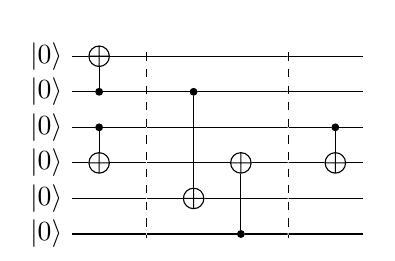
\begin{tikzpicture}
			 \begin{yquant}
			 
			 qubit {$\ket0$} q[6];
	 		cnot q[0] | q[1];
			cnot q[3] | q[2];
			barrier (q);
			
			cnot q[4] | q[1];
			cnot q[3] | q[5];
			barrier (q);
			
			cnot q[3] | q[2];
			 	 
 			\end{yquant}
		\end{tikzpicture}

		\caption{An example of quantum circuit to be compiled}
	\end{center}
\end{figure}

  \begin{figure}[ht]
  	\begin{center}
  		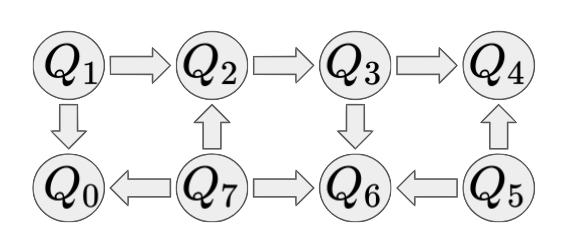
\includegraphics[width=5cm]{img/quantum-processor.png}
		\caption{The connectivity constraints of qubits on a quantum processor}
	\end{center}
\end{figure}
	
 
\subsubsection{Circuit Partitioning into Layers}

 First of all, the given quantum circuit is partitioned into several layers and a layer $l_i$ and all the quantum gates in a single layer $l_i$ do not share any qubits. Also, the number of the depth of a circuit is same as that of layers in the same circuit.
 
 After that, the qubit mapping is proposed in each layer $l_i$ and it does not have to correspond with that of the previous layer  $l_{i-1}$. Instead, a new layer of SWAP gates $\pi_i$ is inserted before the quantum compiler goes onto the next layer. In other words, the sequence of layers will be denoted as $l_0 \pi_1 l_1\pi_2 l_2 \dots$.
 
\subsubsection{Determining the Qubit Mapping}

The quantum compiler determines the mapping relationship between program qubits onto physical qubits on an actual quantum processor for each layer $l_i$, which is denoted as $\sigma^i_j: \{q_0, q_1, q_2, \dots q_{n-1}\} \rightarrow \{Q_0, Q_1, Q_2, \dots Q_{m-1}\}$. ($j$ is a unique id for that relationship, $n$ is the number of qubits on the given program, and $m$ is the number of physical qubits on a quantum processor) This relationship has to satisfy the CNOT-constraints on that hardware and the initial mapping is same of that of the previous layer, in other words, $\sigma^{i-1} = \sigma^i_0$.  The goal of this step is to find $\sigma^{i}$, which is the (sub-)optimal mapping relationship by adding minimum number of new operations by using an algorithm $A^{*}$ search.

\subsubsection{A* Search}
$A^{*}$ search is a state-space-based search algorithm that can be applied to states whose relationships have a tree structure.  The cost of the next node from the root to the node $x$ is $f(x)$, and $g(x)$ is the cost of the path from the root to the current state, and $h(x)$ is the additional cost of the link between the current state and the next state. 

Therefore, $$f(x) = g(x) + h(x)$$

In the case of quantum compilation, the cost of the root state, which is the initial qubit mapping is 0. If the cost for the current state is $f(x)$, $g(x)$ is that of the previous mapping, and the $h(x)$ is the cost for additional layers.

If the current mapping $\sigma^i_j$ is followed by the next mapping  $\sigma^i_h$, the cost of the current mapping would be
$$ f(\sigma^i_j) = f(\sigma^i_j) + 7 \times \textrm{(number of SWAP gates)} $$
The equation above contains 7, because a single SWAP gate requires 7 elementary gates.

\begin{figure}[ht]
	\begin{center}
		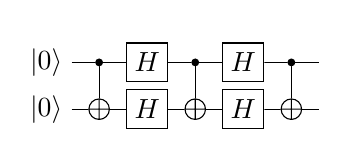
\begin{tikzpicture}
			 \begin{yquant}
			qubit {$\ket0$} q[2];
	 		cnot q[1] | q[0];
			h q[0];
			h q[1];
			cnot q[1] | q[0];
			h q[0];
			h q[1];
			cnot q[1] | q[0];
			\end{yquant}
		\end{tikzpicture}
		\caption{7 elementary gates to implement a SWAP gate}
	\end{center}
\end{figure}

If you assign physical qubits $Q_c$ as a control qubit and $Q_t$ as a target qubit for a CNOT gate $g \in l_i$.  If the shortest directed path between $Q_c$ and $Q_t$ is denoted as $\hat{p}$, the additional gate cost for the CNOT gate $g$ in the current mapping $\sigma^i_j$ would be $$h(g, \sigma^i_j) = 7 \times (\hat{p} - 1)$$.

Therefore, the gate cost of additional layer $l$, which is $h(\sigma^i_j)$ is

$$ h(\sigma^i_j) = max_{g \in l} h(g, \sigma^i_j)$$

\subsubsection{Further Optimization}

In order to perform further optimization, the quantum compiler can incoroperate the information of not only the current layer, but also that of the next layer.  For example, the cost of the current layer can be 
$$ h(\sigma^i_j) = max_{g \in l_i \cup l_{i+1}} h(g, \sigma^i_j)$$

\newpage

\section{Distributed Computing}

 Distributed computing is the study of distributed system, which is a collection of several processors that are connected via network in order to solve a problem whose scale is much larger than what an individual processor can handle.  This type of computation involves message-passing between two physically separated processors to communicate and cooperate with each other by using pure HTTP, RPC, or message queues. \cite{distributedcomputingtext} 
 
 \subsection{Characteristics of Distributed System}
 \par Distributed system has the following characteristics, which are,
 
 \begin{itemize}
 
      \item No common physical clock 
      
      This is the key feature of distributed system because the clock of each processor runs at a different rate, so no clock can keep synchronized even after a single physical clock cycle.  Instead, distributed system depends on logical clock, which is common time platform for the whole system.
      
     \item No shared memory
     
     Each processor in a distributed system has its own memory space, rather than the common physical memory.  This feature indicates that a distributed system does not share its global state.
     
     
      \item Geographical separation
      
      The processors in a distributed system is located in different places, but they do not have to communicate with wide area network (WAN).  Actually, the network of workstations (NOW) and the cluster of workstations (COW) are becoming increasing popular because companies can easily purchase cost-efficient, high-speed, and ready-made processors. 
      
     \item Autonomy and heterogeneity
     
     A distributed system can work together even if it contains various processors which have different size, speed and operating system as long as they cooperate with one another.  This situation is regarded as "loosely-coupled".
     
\end{itemize}

\subsection{Advantages Over Computation by a Single Processor}

Performing computation in a distributed manner provides the following advantages.

\begin{itemize}
 
     \item{Computation by more than one entity}
     
     Applications such as money transfer (client-server) and reaching consensus among parties that are geographically separated (peer-to-peer) require information processing system that each processor can work together.
     
     \item{Resource sharing}
     
     Resource such as data in databases cannot be replicated because it is impossible or at least cost effective. Furthermore, allocating all the resource in just a single server is also not practical because the whole application would become unavailable if the server fails.  In order to solve these potential problems, the whole dataset is usually partitioned into several servers so that it can achieve more rapid access and higher reliability.
     
     \item{Access to geographically remote data and resources}
     
     Copying the whole dataset to every site is not desirable due to not only its predicted high cost, as I mentioned in the previous section, but also too sensitive.  Therefore, these large amount sensitive information, like user information collected by multinational cooperations are stored only in their central data centers and their oversea branches are only allowed to query them.
     
     \item{Enhanced reliability}
     
     Distributed system offers increased reliability due to its ability to replicate resource and achieve simultaneous execution of its given tasks. Also geographically distributed resources are highly unlikely crash or malfunction at the same time under normal circumstance.   This eliability entails several aspects.
     
     \begin{itemize}
     
      	\item{Availability}
	
	Resource become accessible at all times
	
      	\item{Integrity}
	
	The value and state of the resources should be always correct, especially users get concurrent access to those resources.	
	
      	\item{Fault-tolerance}
	
	Distributed system should be able to recover from its failure such as one of its server accidentally shutting down
	
    \end{itemize}
    
    
   \item{Increased performance / cost ratio}
   
     By resource sharing and access to geographically distant data, the performance and cost ratio of distributed system will improve more than using special parallel machines, this is particularly true of the NOW (network of workstation) setting.
     
\end{itemize}

\subsection{Task Allocation Problem}

Here are some definitions of the task allocation problem in distributed system. \cite{definition}
Given a distributed system $G = <V, E>$, where V is the set of nodes and E is the set of communication link between two different nodes, i.e. $\forall v_i. v_j \in V, \exists <v_i, v_j> \in E$.  The set of the resources in $a_i$ is $R_{a_i}$ and that required by the task $t$ is $R_t$.

\begin{enumerate}
	\item{$R_t \subseteq$ $\bigcup_{\forall a_i \in A_t} R_{a_i}$}
	\item{The objective should be either minimizing the execution time \cite{time} or maximizing reliability \cite{reliability}}
	\item{The nodes in $A_t$ can execute the allocated task under the constraint of the network structure $\forall a_i, a_j \in A_t \Rightarrow P_{ij} \subseteq E$ where $P_{ij}$ denotes the path between $a_i$ and $a_j$}
\end{enumerate}

Task allocation is known to be a NP-problem. \cite{np}

\subsection{Distributed Task Allocation Algorithms}

Due to the fact that task allocation problem is classified as NP-hard, many works have proposed heuristic functions for distributed task allocations in various settings.  Here, the author is going to introduce a simple objective function presented in the paper \cite{algorithm}, which is this work is based on.

It is assumed that a multicomputer system consists of $N$ heterogeneous processors with some amount of computational power and the size of memory.  Also, the given program includes $M$ communicating tasks, which is the nodes in the task interaction graph $G(V, E)$ ($V$ is $M$ communicating tasks and E is a set of communication relationship between two tasks).

The objective of this task allocation is to minimize the total execution time. In other words, the author has to come up with the optimal allocation $A$, which $A(i) = p$ indicates that the task $i$ is allocated to the processor $p$ and $TASKS_p$ is a group of tasks that are allocated to a processor $p$.

 The total execution in the heterogeneous computing cluster is same as the execution time in the most heavily loaded processor.  Two main types of costs should be considered.
 
 One is the execution cost.  The execution load in the processor $p$ is the cost of processing all the tasks that are assigned to $p$ for the allocation $A$. Suppose $C_{ip}$ is the cost of processing the task $i$ on the processor $p$, then the total execution cost on the processor $p$ is $$EXEC_p = \sum_{task \in  TASKS_p} C_{task, p}$$
 
  The other cost is the communication cost, which can be calculated by the following formula.
  
  $$COMM_p = \sum_{task \in TASKS_p} \sum_{(i=j), \\(i, j) \in E , \\ A(j) \neq p} d_{ij} * cc_{avg}$$. $d{ij}$ is the data sent between two communicating tasks between $i$, $j$ and $cc_{avg}$ is the average amount of transferring a data unit through the network transmission media.
  
 Therefore, the total cost for the processor $p$ is $$COST_p = EXEC_p + COMM_p$$.
 Because the total execution time is equal to the execution of the most heavily loaded processor, the total execution time can be described as following.
 $$ COST =  max \{COST_p | 1 \leq p \leq n\}$$
 
 Therefore, the object function is $$min \,\,COST$$

\subsection{Models of Process Communication}

There are two basic models of process communication. One is \textit{synchronous} communication, which the sender process blocks its execution until it receives "acknowledgement " (or "ack" in short) from the receiver, which indicates that the receiver accepted the delivered message. In other words, the sender and receiver synchronize with each other, in order to adjust their timings to cooperate.
\par On the other hand, the other model, which is \textit{asynchronous} execution does not require synchronization between the sender and the receiver.  Therefore, the sender executes its following task right after it delivers its message to the receiver. 

\newpage

\section{Distributed Quantum Computing}
 
  Performing quantum computation on a cluster of middle-sized quantum processors is an easier approach compared to build a large single processor due to its lower physical requirement to build each processor \cite{distributedquantumcomputing}.  \\
This chapter explains several components that consists of distributed quantum computing system.

\subsection{Distributed Quantum Algorithms}

Distributed version of Shor's algorithm \cite{distributedshor} and Grover's algorithm \cite{distributedgrover}, both of which takes remote CNOTs (which will be discussed in a  later subsection) were presented in 2004 and 2012, respectively. 
However, the quantum circuits shown in these studies are physical ones, in other words, something that will be implemented directly on physical hardware, not something that users will implement in their programs. 

\subsection{Quantum Compiler for Distributed Quantum Computing}

 Quantum compiler is a software to optimize a quantum circuit defined in the given program to reduce the number of quantum gates and alleviate the effect of physical noise on that quantum state, and map that to the real hardware so that it will satisfy the connectivity constraint on that hardware \cite{qubitallocation}.  Just like the case of a local quantum software, distributed quantum computer also needs its distributed version in order to convert some CNOT gates into remote CNOTs and optimize both its execution time and the number of quantum gates in total, especially that of non-local operations.  This work focuses on the methodology to optimize the total execution time over the distributed quantum computing setting.
 
 \subsection{Gate-Teleportation-Based Non-Local CNOT}
 
Non-local operations are controlled operations between two qubits on two different processors there are three main approach to achieve them.

The first operation is the gate teleporation approach, and is also called non-local quantum gates \cite{gateteleportation} and telegate \cite{arithmetic}.  Here is the quantum circuit that achieve this operation.

Suppose that a person would like to apply a non-local CNOT between $|a_0\rangle$ on one processor and $|b_0\rangle$ on the other processor.  In order to do this, he has to prepare a new bell pair between these two processors.  ($|p_i\rangle$ in the following circuit diagram comes from p in $|\psi (psi)^+\rangle$)

 \begin{figure}[ht]
  	\begin{center}
  		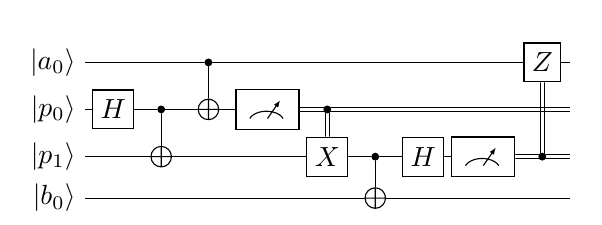
\begin{tikzpicture}
   			\begin{yquant}
      				qubit {$\ket{\reg_{\idx}}$} a[1];
     				 qubit {$\ket{\reg_{\idx}}$} p[2];
     				 qubit {$\ket{\reg_{\idx}}$} b[1];
      				h p[0];
      				cnot p[1] | p[0];
      				cnot p[0] | a[0];
      				measure p[0];
      				x p[1] | p[0];
      				cnot b[0] | p[1];
      				h p[1];
      				measure p[1];
     				z a[0] | p[1];
   			\end{yquant}
		\end{tikzpicture}
		\caption{Quantum circuit for a non-local CNOT gate}
	\end{center}
\end{figure}

\newpage 

\subsection{Quantum Teleportation}

  Unlike classical communication, quantum states cannot be just copied and transmit to other nodes due to the no-cloning theorem, which forbids duplication of any quantum state.  However, a method called quantum teleportation \cite{teleportation} was proposed, which overcomes the restriction and allows sender to transmit single qubit state to a distant location. 
 		
This method requires both the single qubit state and a new Bell pair, and also the sender have to prepare two qubits and the receiver have to prepare one qubit.  After applying a CNOT gate and an H gate in the figure above, the sender have to measure both qubits and send those measurement results over the classical network.  After the receiver get those measurement results and apply some quantum gates if the measurement results of corresponding qubits on the sender's side are 1, in order to correct on the quantum state on the receiver's side.

\begin{figure}[ht]
  	\begin{center}
  		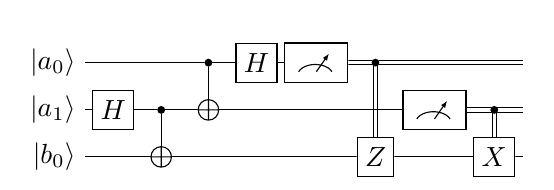
\begin{tikzpicture}
			\begin{yquant}
	 			qubit {$\ket{\reg_{\idx}}$} a[2];
	 			qubit {$\ket{\reg_{\idx}}$} b[1];	 
	 			h a[1];
	 			cnot b[0] | a[1];
	 			cnot a[1] | a[0];
	 			h a[0];
	 			measure a[0];
	 			z b[0] | a[0];
	 			measure a[1];
	 			x b[0] | a[1]; 	 
 			\end{yquant}
		\end{tikzpicture}
	\caption{Quantum circuit for quantum teleportation}
	\end{center}
\end{figure}

\subsection{Quantum-Teleportation-Based Non-Local CNOT}

 The second approach for performing a non-local CNOT gate is based on quantum teleportation mentioned in the previous section.  This approach assumes that every quantum processor has something called "communication qubits", which is a qubit that serves for communication purpose, unlike those used for computation purpose, which are called "data qubits".
 
 \begin{figure}[ht]
  	\begin{center}
  		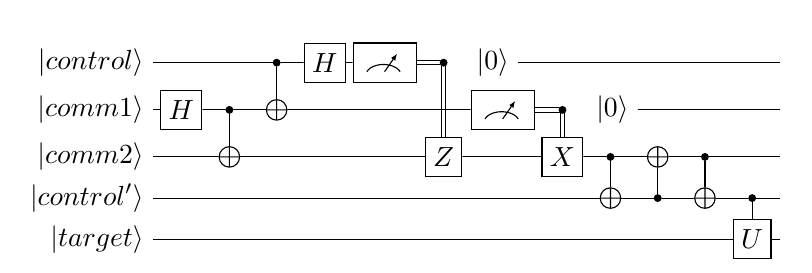
\begin{tikzpicture}
			 \begin{yquant}
			 qubit {$\ket{\reg}$} control[1];
	 		 qubit {$\ket{\reg}$} comm1[1];
	 		 qubit {$\ket{\reg}$} comm2[1];
	 		 qubit {$\ket{\reg}$} control'[1];
	 		 qubit {$\ket{\reg}$} target[1]; 
	 
			 h comm1[0];
			 cnot comm2[0] | comm1[0];
	 		cnot comm1[0] | control[0];
	 		h control[0];
	 		measure control[0];
	 		z comm2[0] | control[0];
	 		discard control;
	 		init {$\ket{0}$} control;
	 		measure comm1[0];
	 		x comm2[0] | comm1[0];
	 		discard comm1;
			 init {$\ket{0}$} comm1;
			cnot control'[0] | comm2[0];
	 		cnot comm2[0] | control'[0];
			cnot control'[0] | comm2[0];
			box {$U$} target[0] | control'[0];
	 
 			\end{yquant}
			\end{tikzpicture}
			\vskip\baselineskip
			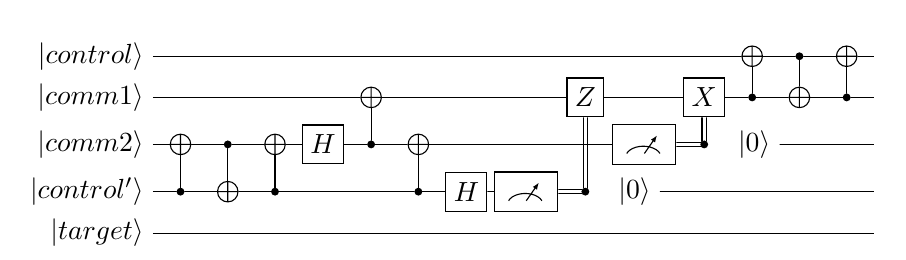
\begin{tikzpicture}
 			\begin{yquant}
			qubit {$\ket{\reg}$} control[1];
	 		qubit {$\ket{\reg}$} comm1[1];
	 		qubit {$\ket{\reg}$} comm2[1];
	 		qubit {$\ket{\reg}$} control'[1];
	 		qubit {$\ket{\reg}$} target[1]; 
	 
	 		cnot comm2[0] | control'[0];
	 		cnot control'[0] | comm2[0];
	 		cnot comm2[0] | control'[0];
	 
	 		h comm2[0];
	 		cnot comm1[0] | comm2[0];
	 		cnot comm2[0] | control'[0];
	 		h control'[0];
	 		measure control'[0];
	 		z comm1[0] | control'[0];
	 		discard control';
	 		init {$\ket{0}$} control';
	 		measure comm2[0];
	 		x comm1[0] | comm2[0];
	 		discard comm2;
	 		init {$\ket{0}$} comm2;
	 
	 		cnot control[0] | comm1[0];
			cnot comm1[0] | control[0];
			cnot control[0] | comm1[0];
	 
 			\end{yquant}
		\end{tikzpicture}

		\caption{The full quantum circuit for a teledata non-local controlled-U gate}
	\end{center}
\end{figure}
	
\newpage

\subsection{Data-Qubit-Swapping-Based Non-Local-CNOT}

The last approach for the non-local CNOT gate aims to sort qubits in the quantum processors so that each CNOT gates would be executed on the neighboring processors. (the paper \cite{distributedquantumcompiler} assumes linear topology)

\begin{figure}[ht]
  	\begin{center}
  		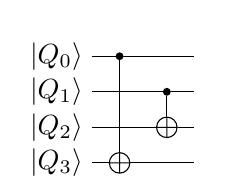
\begin{tikzpicture}
 			\begin{yquant}
 
			qubit {$\ket{\reg}$} Q_0[1];
			qubit {$\ket{\reg}$} Q_1[1];
			qubit {$\ket{\reg}$} Q_2[1];
			qubit {$\ket{\reg}$} Q_3[1];

			cnot Q_3[0] | Q_0[0];
			cnot Q_2[0] | Q_1[0];
			\end{yquant}
		\end{tikzpicture}

		\caption{The quantum circuit before the data qubit swapping occurs}
	\end{center}
\end{figure}
	
\begin{figure}[ht]
  	\begin{center}
  		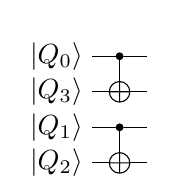
\begin{tikzpicture}
			\begin{yquant}
 
			qubit {$\ket{\reg}$} Q_0[1];
			qubit {$\ket{\reg}$} Q_3[1];
			qubit {$\ket{\reg}$} Q_1[1];
			qubit {$\ket{\reg}$} Q_2[1];

			cnot Q_3[0] | Q_0[0];
			cnot Q_2[0] | Q_1[0];

 			 \end{yquant}
		\end{tikzpicture}
		\caption{The quantum circuit after the data qubit swapping occurs}
	\end{center}
\end{figure}	

\begin{algorithm}
 \caption{Algorithm for Data-Qubit Swapping}
 \begin{algorithmic}[1]
  \Require n-qubit circuit layer L with mod(n, 4) = 0 and $\frac{n}{2}$ CNOTs
  \Ensure  layer L with each CNOT operating on neighbor qubits
 \Function {Sort}{L}
    \If {$\exists \, CNOT(q_i, q_j)$ with $i, j \leq \frac{n}{2}$} 
   	\State{// $\exists \, CNOT(q_k, q_l)$ with $k, l > \frac{n}{2}$}
	\State{SWAP ($q_{i+1}$, $q_j$)}
	\State{SWAP($q_{k+1}$, $q_l$)}
	\State{L = L \textbackslash \{$q_i$,  $q_{i+1}$,  $q_{k}$,  $q_{k+1}$\}}
    \Else
	\State{// $\exists \, CNOT(q_{\frac{n}{2}}, q_l)$ with $l > \frac{n}{2}$}
	\State{// and $\exists \, CNOT(q_i, q_{l-1})$ with $i < \frac{n}{2}$}
	 \State{SWAP ($q_{\frac{n}{2}}$, $q_{l-1}$)}
	  \State{SWAP ($q_i$, $q_{\frac{n}{2}-1}$)}
	  \State{L = L \textbackslash \{$q_{\frac{n}{2}-1}$,  $q_{\frac{n}{2}}$,  $q_{l-1}$,  $q_{l}$\}}
    \EndIf
    
    \If {$L \neq \emptyset$}
    	\State{Sort(L)}
    \EndIf
    
\EndFunction

 \end{algorithmic} 
 \end{algorithm}

\newpage

 \subsection{Quantum Processor}
  A quantum processor, which corresponds to individual processor in a classical distributed system, has several qubits and links between two qubits in a limited topology.
  
  \begin{figure}[ht]
  	\begin{center}
  		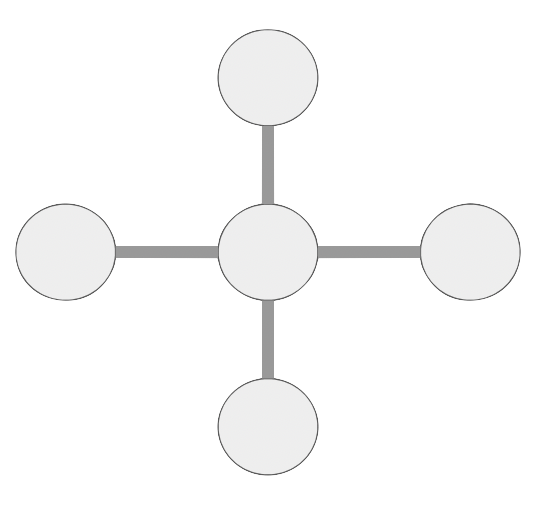
\includegraphics[width=5cm]{img/processor.png}
		\caption{An example of the layout of a quantum processor}
	\end{center}
\end{figure}
	
Usually, qubits in a current quantum processor are connected with a few neighboring qubits due to its physical restriction on a hardware.  Also, the error rate of a CNOT gate is much higher than that of a single quantum gate.
 
 \subsection{Communication Link for Distributed Quantum Computing}
Networking between two quantum processors need two types of communication links, which are classical links that transmit measurement results in the process of either telegate or teledata non-local CNOT gate, and quantum links that prepare create entanglement between the two qubits between the two neighboring quantum processors, or communication qubits of both processors.    

%\end{document}
%%% Local Variables:
%%% mode: japanese-latex
%%% TeX-master: "../thesis"
%%% End:
\chapter{Related Works}
\label{related works}

\section{Performance of  An Interprocessor CNOT Gate}
Both the execution time and required amount of resource for inter-node communication are important because it significantly affects the total execution time and the whole architecture of a distributed quantum computing system. 

 The work \cite{gateteleportation} proved that one bit of classical communication in each direction and one bell pair are sufficient for the non-local CNOT gate.  It also proposes the optimal implementation of a non-local CNOT in terms of communication overhead and the number of required quantum gates. 
 
 The work \cite{arithmetic} compared the performance between "telegate" and "teledata" approach in terms of various number of data qubits, communication qubits, and its network topology.  It presents the fact that the teledata approach is faster than the telegate approach, and that decomposition of a quantum gate will improve the performance.  It also shows that each node should have a few logical qubits and two communication qubits.

\section{Minimization of the Number of Interprocessor Communication}

Dividing the given quantum circuit into several fragments one of the main jobs for a distributed quantum compiler.  In the process of partitioning the given quantum circuit, the distributed quantum compiler has to minimize the number of inter-processor communication in order to reduce the delay in the entire circuit execution.  

The work \cite{exhaustivesearch} proposed an exhaustive-search-based algorithm to find a partition of the given quantum circuit with the minimum number of quantum teleportation between two quantum processors.

The work \cite{hypergraph} applied the heuristic algorithm for a hypergraph partitioning problem in order to minimize the number of inter-processor communication, which can be applied to more than two quantum processors.

The work \cite{genetic} tackled the minimization of interprocessor communication by using the genetic algorithm and demonstrated its advantage over random search over the search space.

The work \cite{dynamic} converted the given quantum circuit into a bi-partite graph and the gates and qubits are assigned to each part of the graph.  Then, the graph was partitioned into $K$ parts which minimizes the number of non-local CNOTs.

The work \cite{Kernighahn-Lin} used the Kernighahn-Lin algorithm, which is one of the heuristic algorithms for the graph partitioning problem, to find arbitrary number of partition with the smallest number of interprocessor communication.

The work \cite{WQCP} proposed a new scheme for reducing interprocessor communication called window-based quantum circuit partitoning, or WQCP in short.  This approach combined reduction of both telegate and teledata opportunities. 

The work \cite{matrix} suggested another algorithm for minimizing the interprocessor communication which consists of two phases by using the connectivity-matrix-based representation of a quantum circuit.
In the first phase, it proposed two objective functions to minimize the number of non-local CNOTs and difference between the number of qubits in two partitioning.  In the second phase, two heuristics were also proposed two other heuristics to minimize the number of quantum teleportation required.

\section{Quantum Compiler For Distributed Quantum Computing}

The work \cite{distributedquantumcompiler} discussed the design of a general-purpose, efficient, and effective distributed quantum computer. General purpose means no assumption about the given quantum circuit. Efficient means polynomial time complexity that grows polynomially with the number of qubits and linearly with the circuit depth.  Effective assures a polynomial worst-case overhead in terms both depth of the compiled circuit, the number of entanglement generation.

 This study also derived the analytical upper bound of the circuit depth both for the entanglement-based non-local operation and the data-qubit-swapping-based non-local operation.
 
 The depth overhead of the entanglement-swapping-based strategy would be at most 
 
  \begin{equation}
 \frac{n}{2}d_{es}
  \end{equation}
  
 \begin{equation}
 d_{es} = c_{le} + c_{bsm} + c_{cx}
  \end{equation} 
 
  On the other hand, the depth overhead of the data-qubit-swapping strategy is
  
   \begin{equation} 
  \frac{n}{4}d_{qs} + d'_{qs}
   \end{equation} 
   
   \begin{equation} 
   d_{qs} = 3(c_{le} + c_{bsm} + c_{cx})
    \end{equation}
    
  \begin{equation}
   d'_{qs} = c_{le} + c_{cx}
   \end{equation}
  
  $n$ is the number of qubits, $c_{le}$ is the number of layers required to perform the link entanglement, $c_{bms}$ is that to perform entanglement swapping, $c_{cx}$ is that to perform remote CNOTs.
  This study mentions that parameters $c_{le}$, $c_{bms}$, $c_{cx}$ heavily depends on the underlying hardware architecture.
  
  It also compare the performance of both strategies with the previous work \cite{hypergraph}.  It experimentally demonstrated that the entanglement-swapping-based strategy requires less number of layers for link generation, and the data-qubit-swapping-based strategy requires less circuit depth, on the worst network topology (the linear topology with one qubit on an each processor).


%%% Local Variables:
%%% mode: japanese-latex
%%% TeX-master: "./thesis"
%%% End:

\chapter{Problem Definition and Proposal}
\label{problem_definition_and_proposal}

This chapter explains a new problem about the qubit allocation in the \\ distributed quantum computing system and propose the solution for that problem.

\section{Problem Definition}

 In order to execute distributed computing, a collection of tasks should be allocated onto multiple processors limited by a certain network topology.  These processors might have different properties such as their execution time and their memory size.  Algorithms regarding distributed computing aim to achieve efficiency in terms of either reduction in the total execution time or increase of total reliability compared to the case of execution of the same tasks on the single processor.

Previous works about qubit allocation on a single quantum processor tries to improve the fidelity of the output quantum state even in the presence of physical noise on a hardware, which is "reliability" for quantum computing, and these works can be directly applied to improve the total fidelity even in the case of distributed quantum computing if the whole quantum computing cluster is considered as a single larger-scale quantum processor .

 However, qubit allocation for distributed quantum computing to minimize the total execution time has not been investigated, even though this is one of the two major optimization criteria for task allocation problem in the classical setting. 
 
 This work formulates the problem of qubit allocation on multiple quantum processors with varying execution time as an optimization problem and define its objective function.  It also demonstrates the validity of the proposed method by numerical simulation, which adopted simulated annealing as a heuristic optimization algorithm.
 
\section{Formulation as An Optimization Problem}

Suppose a distributed quantum computing system consists of $N$ quantum processors connected via communication links. Each quantum processor has limited number of qubits and execution time.

A quantum circuit in the program consists of several qubits and $M$ gates, including CNOTs which corresponds to an interaction graph $G(V, E)$. $V$ represents a set of qubits and $E$ represents set of two qubits involved in each CNOT gate.  $q_i \in V$ is labeled by the qubit index, and $(control, target) \in E$ is labeled by control-target relationship of all the CNOT gates.

The problem is how to allocate each qubits in the given quantum circuit to which processor with varying execution time in order to minimize the total execution time. This problem can be formulated as an optimization problem, which requires a cost function, which is the value to either maximize or minimize to acquire the optimal solution.

\section{Objective Function}
Suppose $A$ be the optimal assignment such that $A(q_i) = p_j$ if a qubit $q_i$ in the given quantum circuit to a quantum processor $p_j$. Qubits allocated to a quantum processor $p_j$ is denoted as $qubits_j$, single qubit gates allocated to a qubit $q_i$ is $gates_i$ and the execution time on a quantum processor $q_j$ is $time_j$.

The cost of executing all single-qubit gates on a qubit $q_i$ on a quantum processor $p_j$ is 

 \begin{equation}
\sum_{ \operatorname{gate} \in  \operatorname{gates_i}}  \operatorname{time_j}
 \end{equation}
 
Therefore, the cost of executing all the single-qubit gates on all the qubits allocated on quantum processor $p_j$ is 

 \begin{equation}
\operatorname{GATECOST_j }= \sum_{ \operatorname{qubit} \in  \operatorname{qubits_j}} \sum_{ \operatorname{gate} \in  \operatorname{gates_{qubit}}}  \operatorname{time_j}
 \end{equation}

Suppose a CNOT gate CNOT(control, target) involves two qubits, which are control $\in qubits_s$ and target $\in qubits_t$ and all the CNOT gates in a quantum processor $p_j$ are denoted as $CNOTs_{j}$.

The communication cost in a quantum processor $p_j$ is 

 \begin{equation}
 \operatorname{COMMCOST_j} = \sum_{ \substack{ \operatorname{CNOT} ( \operatorname{control},  \operatorname{target}) \in  \operatorname{CNOTs_{j}} \\  \operatorname{control} \in  \operatorname{q_s} \\  \operatorname{target} \in  \operatorname{q_t}}} pathlength(s, k)
 \end{equation}
 
pathlengthis the length of the path between the processor $s$ and the processor $t$ on the given network topology, and the processor $j$ is same as at least either the processor $s$ or the processor $t$.

Thus, the total cost on a quantum processor $p_j$ is 

 \begin{equation}
 \operatorname{COST_j} =  \operatorname{GATECOST_j} +  \operatorname{COMMCOST_j}
 \end{equation}

Both execution of single qubit gates and communication with other processors affect the total execution time on each processor, and because the processor with the greatest cost will decide the total execution time on the whole distributed quantum system, the following value should be calculated.

 \begin{equation}
 \operatorname{MAXCOST} = \max \{ \operatorname{COST_j} | 1 \leq j \leq N\}
 \end{equation}

Also, minimizing this value will reduce both the execution time for quantum gates execution and interprocessor communication, and the objective function of this problem is 

 \begin{equation}
  \operatorname{min}\, \operatorname{MAXCOST}
  \end{equation}
  
  In the chapter 5, the optimization of this proposed objective function is performed by one of the most popular heuristic optimization algorithm called simulated annealing, which will be explained in the following section.

\newpage

\section{Simulated Annealing}
Simulated annealing is a heuristic algorithm which reaches to the global optimal solution in some cases \cite{simulatedannealing, Boltzmann}. Its idea comes from cooling the molten metal until it gains crystal structure, so it calculates the values of "temperature", which how long the optimization has been executed and "energy" which evaluates how close the current answer is to the optimal solution.  The algorithm starts with high temperature and energy, and as the temperature becomes lower,  the solution changes randomly and the combination and the answer after randomization process is accepted even its energy becomes higher than its previous answer in order to avoid being stuck in the local minimum.

Here is the pseudocode for the simulated annealing algorithm.

\begin{algorithm}
 \caption{Simulated Annealing}
  \begin{algorithmic}[1]
  \Require A random allocation A, temperature T, iteration number IterNum
  \Ensure The optimal allocation A'
 \Function {SimulatedAnnealing}{A, T, IterNum}
  \State{A' = A}
 \For {iter := 1 to IterNum}
     \State{temp := $\operatorname{T} * (1- \operatorname{iter/IterNum})$}
     \State{copyA $\leftarrow$ copy(A')}
     \State{newA $\leftarrow$ move(copyA)}
     \State{eng $\leftarrow$ calc\_energy(copyA)}
     \State{neweng $\leftarrow$ calc\_energy(newA)}
     \If {accept\_prob(eng, neweng, temp) $>$ randomvalue(0, 1)}
     	\State{A' = NewA}
    \EndIf
 \EndFor
       \State {return  A'}
\EndFunction
 \end{algorithmic}
 \end{algorithm}
 
 \begin{algorithm}
 \caption{Finding a neighbor state}
  \begin{algorithmic}[1]
\Require Processor list P $\{\operatorname{P_0}, \operatorname{P_1}, \dots \operatorname{P_N}\}$, initial allocation A  $\{\operatorname{P_0}:\operatorname{qubits_0}, \operatorname{P_1}:\operatorname{qubits_1}, \dots \operatorname{P_n}:\operatorname{qubits_n}\}$
 \Ensure New allocation A
 \Function {move}{}
 \State{$\operatorname{P_i}$ $\leftarrow$ a randomly selected processor}
 \State{$\operatorname{P_j}$ $\leftarrow$ another randomly selected processor}
 \State{$\operatorname{qindex_i}$ $\leftarrow$ a randomly selected qubit index from 0 to $\operatorname{len(qubits_i)}$}
 \State{$\operatorname{qindex_j}$ $\leftarrow$ a randomly selected qubit index from 0 to $\operatorname{len(qubits_j)}$}
\State{$\operatorname{A[P_i][qindex_i]}$, $\operatorname{A[P_j][qindex_j]}$ = $\operatorname{A[P_j][qindex_j]}$, $\operatorname{A[P_i][qindex_i]}$}
\EndFunction
 \end{algorithmic}
 \end{algorithm}
  
 \begin{algorithm}
 \caption{Calculating the energy value}
  \begin{algorithmic}[1]
 \Require initial allocation $\operatorname{A}$  $\{\operatorname{P_0}: \operatorname{qubits_0}, \operatorname{P_1}: \operatorname{qubits_1}, \dots \operatorname{P_n}: \operatorname{qubits_n}\}$, a quantum gate list $\operatorname{gate\_list}$ $\{\operatorname{gate_0}, \dots, \operatorname{gate_N}\}$, an execution time list $\operatorname{time\_list}$ [$\operatorname{time\_0}, \dots \operatorname{time_N}$], network topology N
 \Ensure An energy value $E$
 \Function {calc\_energy}{A, $\operatorname{gate\_list}$}
\State{$\operatorname{processor\_list}$ $\leftarrow$ $\operatorname{[keys\,in\,A]}$}
 \State{$\operatorname{gate\_cost\_list}$ $\leftarrow$ $\operatorname{[0\,for\,processor\,in\,processor\_list]}$}
 \State{$\operatorname{comm\_cost\_list}$ $\leftarrow$ $\operatorname{[0\,for\,processor\,in\,processor\_list]}$}
 \For {$\operatorname{processor\_id}$ := $0$ to $\operatorname{length\,of\,processor\_list} - 1$}
 	\For {$\operatorname{gate}$ := $\operatorname{gate_0}$ to $\operatorname{gate_N}$}
		\If{$\operatorname{gate\_name} \neq$ CNOT and $\operatorname{gate\_index} \in$ A[processor\_id]}					
		\State{$\operatorname{gate\_cost\_list[processor\_id]}$ += $\operatorname{time\_list[processor\_id]}$}
		\EndIf
	\EndFor
 \EndFor
 \State{$\operatorname{distance\_matrix} \leftarrow \operatorname{N\_distance\_matrix}$}
 \For {$\operatorname{processor\_id}$ := $0$ to $\operatorname{len(processor\_list)} - 1$}
 	\For {$\operatorname{gate}$ := $\operatorname{gate_0}$ to $\operatorname{gate_N}$}
		\If{$\operatorname{gate\_name}$ = CNOT}
			\If{$\operatorname{gate\_index, gate\_target\_index} \in\operatorname{A[processor\_id]}$} 
				\State{$\operatorname{comm\_cost\_list[processor\_id]}$ += $0$}
			\ElsIf{$\operatorname{gate_index} \in \operatorname{A[processor\_id]}$}
				\For{$\operatorname{processor'\_id} := 0$ to $\operatorname{length\,of \,processor\_list} - 1$}
					\If{$\operatorname{gate\_target\_index} \in \operatorname{A[processor'\_id]}$} 
					\State{$\operatorname{distance}  \leftarrow \operatorname{distance\_matrix[processor\_id][processor'\_id]}$}
					\State{$\operatorname{comm\_cost\_list[processor\_id]}$ += $\operatorname{distance}$}
					\EndIf
				\EndFor
			\ElsIf{$\operatorname{gate_gate\_index} \in\operatorname{A[processor\_id]}$}
				\For{$\operatorname{processor'\_id} := 0$ to $\operatorname{length\,of\,processor\_list} - 1$}
					\If{$\operatorname{gate_index} \in \operatorname{A[processor'\_id]}$} 
					\State{$\operatorname{distance} \leftarrow \operatorname{distance\_matrix[processor'\_id][processor\_id]}$}
					\State{$\operatorname{comm\_cost\_list[processor\_id]}$ += $\operatorname{distance}$}
					\EndIf
				\EndFor
			\EndIf
		\EndIf
	\EndFor
 \EndFor
 
 \For {$\operatorname{processor\_id}$ := $0$ to $\operatorname{length\,of\,processor\_list} - 1$}
 	\State{$\operatorname{gate\_cost}  \leftarrow \operatorname{gate\_cost\_list[processor\_id]}$}
	\State{$\operatorname{comm\_cost}  \leftarrow \operatorname{comm\_cost\_list[processor\_id]}$}
 	\State{$\operatorname{cost\_list[processor\_id]} \leftarrow \operatorname{gate\_cost + comm\_cost}$}
\EndFor
\State {return $\operatorname{\max cost\_list}$}
  \EndFunction 
 \end{algorithmic}
 \end{algorithm}
 \newpage
 \begin{algorithm}
 \caption{Calculating the acceptance probability}
  \begin{algorithmic}[1]
  \Require current energy value $\operatorname{cur\_eng}$, new energy value $\operatorname{new\_eng}$, current temperature $\operatorname{temp}$
  \Ensure an acceptance probability $prob$
  \Function {accept\_prob}{cur\_eng, new\_eng, temp}
 	\If {$\operatorname{cur\_eng}$ $<$ $\operatorname{new\_eng}$}
		\State{return $1$}
	\Else
		\State{return $\operatorname{\exp{(-(new\_eng - cur\_eng)/temp)}}$}
	\EndIf
   \EndFunction 
  \end{algorithmic}
 \end{algorithm}


%%% Local Variables:
%%% mode: japanese-latex
%%% TeX-master: "../bthesis"
%%% End:

\chapter{Evaluation}

 In this chapter, the author investigates the efficiency of the allocation method proposed in the previous chapter, under the distributed quantum computing system with several processors with different number of qubits, different execution time, and the limited network topology.  The following experiments compare the total execution time in each setting among the case of random allocation, the case when only the gate cost is optimized, the case when only the communication cost is optimized, and the case when both costs are optimized.
  
  These experiments were performed by a distributed quantum computing simulator called HeqSim(Heterogeneous Quantum Computing Simulator) \cite{heqsim} that I have developed.
  
\section{Experiment Settings}
 
 Here are the details of the setting of each experiment.
 
\begin{table}[htb]
\centering
  \caption{The details of all experiment settings}
 \begin{tabular}{|c|c|c|c|} \hline
 	\# of Experiment & \# of Processors & \# of total qubits & Network topology \\ \hline
	1 & 2 & 6 & linear \\ \hline
	2 & 4 & 8 & linear \\ \hline
	3 & 4 & 8 & ring \\ \hline
	4 & 4 & 8 & star \\ \hline
	5 & 4 & 8 & random \\ \hline
 \end{tabular}
 \end{table}
 
 \newpage
 
 \section{Experiment 1: Qubit Allocation to Two Quantum Processors}
 
 The first experiment is the simplest one, which is allocation of qubits onto two quantum processors that are connected with each other,  and each processor has different number of qubits and gate execution time.
 
 \begin{figure}[h]
  		\begin{center}
  			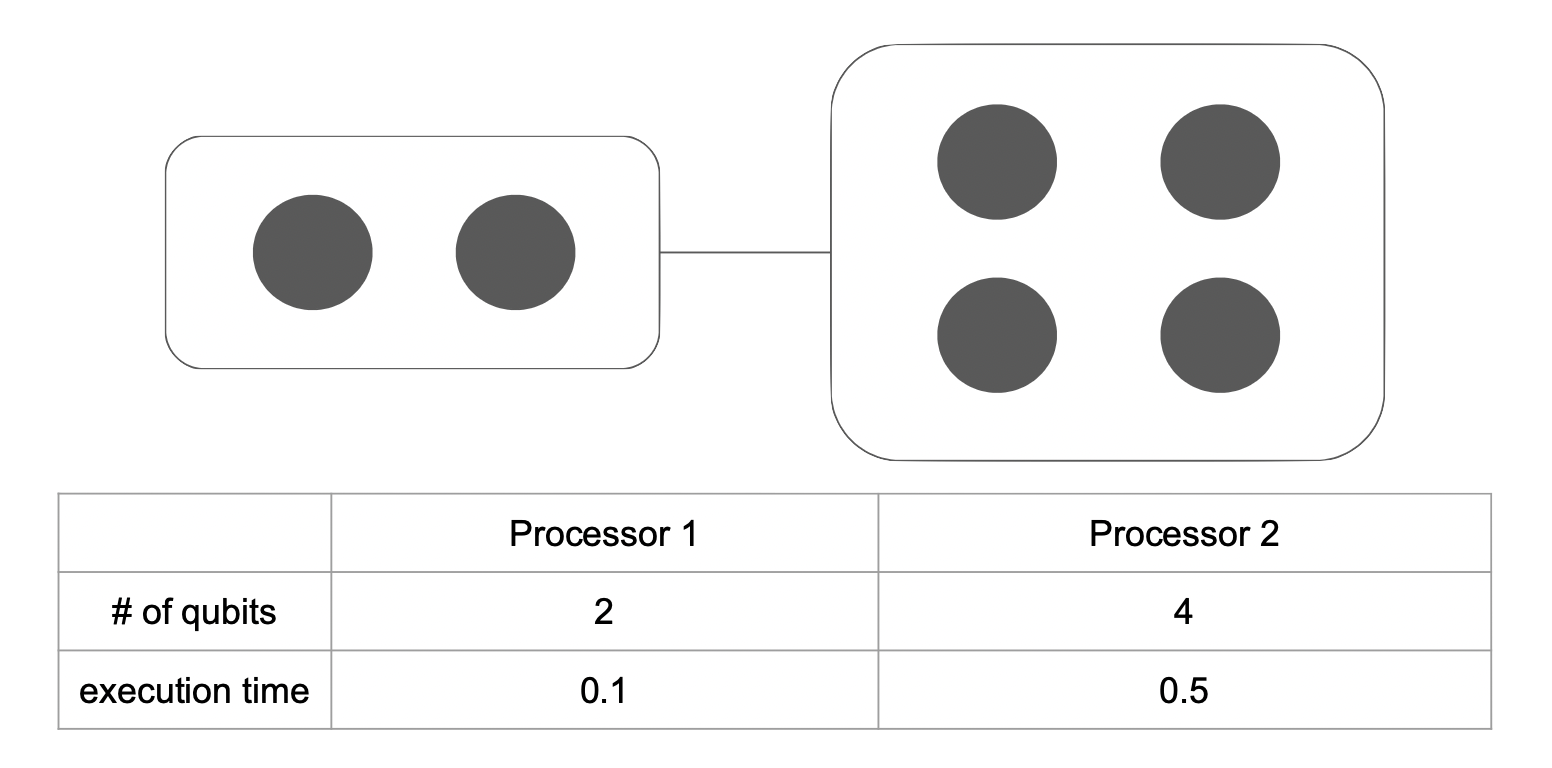
\includegraphics[width=8cm]{img/first_experiment.png}
			\caption{The details of each quantum processor}
			\label{Fig4}
		\end{center}
	\end{figure}
 
 The author executed the following circuit on these two quantum processors.  This circuit is a quantum circuit for solving 6-qubit Simon's problem and also a part of the set of quantum circuits that can be used for benchmarking purpose[20]. 
 \newline
 \newline
 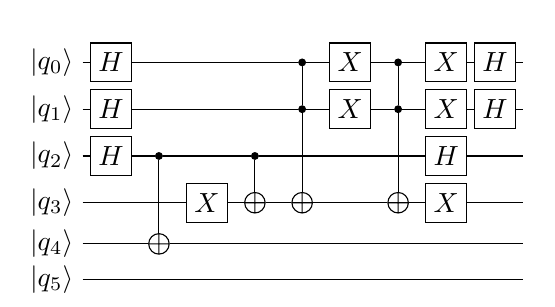
\begin{tikzpicture}
   \begin{yquant}
      qubit {$\ket{\reg_{\idx}}$} q[6];
      
      h q[0];
      h q[1];
      h q[2];
      cnot q[4] | q[2];
      x q[3];
      cnot q[3] | q[2];
      cnot q[3] | q[0, 1];
      x q[0];
      x q[1];
      cnot q[3] | q[0, 1];
      x q[0];
      x q[1];
      x q[3];
      h q[0];
      h q[1];
      h q[2];
   \end{yquant}
\end{tikzpicture}
  \newline
 \newline
 The author compared the total execution time of three different allocation cases, which are when only the gate execution cost is optimized, when only the communication cost is optimized, and when both costs are optimized.  Here is the outcome of this experiment.  (The value in each case is the average value of 10 different execution)
 \newpage
  \begin{figure}[h]
  		\begin{center}
  			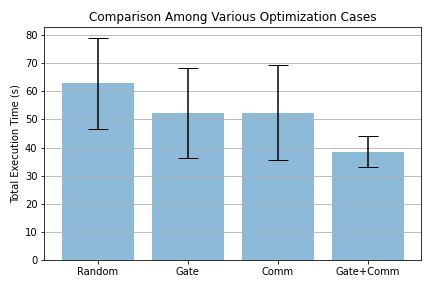
\includegraphics[width=8cm]{img/first_experiment_plot.png}
			\caption{Result of The Experiment 1}
			\label{Fig4}
		\end{center}
	\end{figure}
 
 As you can see in the figure above, the case of random allocation was outperformed by the three other cases, and actually the case when gate execution cost was optimized yielded the best result.
 
\section{Experiment 2: Qubit Allocation to Four Quantum Processors (linear topology)}
\section{Experiment 3: Qubit Allocation to Four Quantum Processors (ring topology)}
\section{Experiment 4: Qubit Allocation to Four Quantum Processors (star topology)}
\section{Experiment 5: Qubit Allocation to Four Quantum Processors (random topology)}

%%% Local Variables:
%%% mode: japanese-latex
%%% TeX-master: "../bthesis"
%%% End:

\chapter{Conclusion}
\label{discussion}

\section{Discussion} 

This thesis aims to propose an effective scheme for qubit allocation for distributed quantum computing to reduce the total execution time, and the chart in the previous chapter clearly demonstrates that the case when the both gate execution cost and communication cost are optimized performs the best.  This fact also states that, similar to the task allocation algorithm for classical distributed computing, people have to take both the task (quantum gate) execution cost and communication cost into account in order to come up with an (nearly-) optimal qubit allocation in terms of reducing the total execution time.

 In this experiment, the total execution time of the gate-cost-based case and that of the communication-cost-based-case are almost the same. However, there are some cases where either the gate-cost-based optimization or the communication-cost-based optimization works better than the other.  For example, gate-cost-based optimization would work better if the given circuit have more single qubit gates than CNOT gates and these gates are fairly allocated to each qubit.  On the other hand, the communication-cost-based optimization yields a better performance if the given quantum circuit has more CNOT gates than one-qubit gates, and each processor has less neighboring processors, such as linear topology.
 
 \section{Significance of This Work}

 This work has two main significance for the field of distributed quantum computing. 
 One is that the scheme proposed in this thesis is the first execution-time-oriented qubit allocation algorithm for distributed quantum computing. 
 
  If the mankind finally overcomes the problem of severe physical noise on each quantum hardware and achieves the large-scale, fault-tolerant, and even distributed quantum computing, they may want to accelerate the whole computing process to achieve more efficient quantum computing. 
  
  In order to speed up the execution of a large-scale quantum circuit with enormous amount of quantum gates on heterogeneous quantum processors, they have to care about both the execution time on each quantum processor and communication cost between each pair of those processors. 
 
 The other significance is that the qubit allocation with the minimum amount of communication is, at least, not always optimal in terms of its total execution time, as I stated in the previous section.
 
 \section{Future Works}
 
 This work only focuses on deciding which qubit should be allocated to which quantum processor, but a few other procedures have to be executed in order to achieve more efficient quantum computing.  For example, after qubits are allocated to each processor, the quantum circuit should be modified to reduce the number of  communication between quantum processors.  Also, similar to the qubit mapping schemes for local quantum processors, the algorithm for choosing which allocated qubit should be mapped to which physical qubit should also be investigated.



%%% Local Variables:
%%% mode: japanese-latex
%%% TeX-master: "./thesis"
%%% End:


\vspace{-5mm}

\nocite{*}
\input{bib/biblio}\thispagestyle{plain}%bibtex

\chapter*{Acknowledgment}
\addcontentsline{toc}{chapter}{Acknowledgment}
\label{thanks}

First and foremost, I would like to show my gratitude to Professor Van Meter for offering me with opportunities to work on various research fields including quantum machine learning, and digital quantum simulation and distributed quantum computing, and make so many mistakes in the first three years. I could not have felt confident about progress of my knowledge and overall capabilities in the last four years if I join in any other research groups.

I also feel grateful to Professor Takahiko Satoh, who have provided me with severe and honest feedbacks about my slides and the way I make a presentation.  Without his patient support, I would not have been able to express my research topic using easy words to those who are not familiar with quantum computing.

I would also like to appreciate Professor  Michal Hajdušek, who allowed me to work on a digital quantum simulation about quantum synchronization between two spin-1 particles.  Even though understanding the setting itself is a really hard work, it is my honor to work on quantum physics, which is my long-time favorite since when I was in high school.  I will resume this joint research after I start my Master's.

I also appreciate Professor Masashi Aono, who taught me the basics of optimization theory and complex system in his lectures.  I would not have thought about working on combinatorial optimization for my graduation thesis, and quantum synchronization for the other research, if I didn't take his intriguing lectures.

I also thank other members in AQUA, especially Ryosuke Satoh for mentoring my research work in this entire year and taking care of me in various aspects, Naphan Benchasattabuse for always giving me critical feedbacks after my progress report, Yasuhiro Okura for suggesting me the details of this research topic, Taaki Matsuo for treating me so many times, Nozomi Tanetani for keeping encouraging me when I felt devastated in the Mitou Target, and Shigetora Miyashita for having a thoughtful conversation about modern physics.

Last but not least, I would like to express my deepest gratitude to my family members who have raised me and become supportive in any situations.  
%%% Local Variables:
%%% mode: japanese-latex
%%% TeX-master: "../yummy_bthesis"
%%% End:

%\appendix
\chapter{Appendix}


\section{付録内容だよ}

書くよ


\end{document}

%%% Local Variables:
%%% mode: japanese-latex
%%% TeX-master: t
%%% End:
